\chapter{Magma Dynamics: porosity waves}
\label{cha:porosity-waves}

\section{Problem Overview}
\label{sec:porosity_waves-formulation}


While many modeling packages in Earth science solve for thermal or
thermo-chemical convection,  one of the strengths of \TF{} is that it
is not a ``convection code'' or a ``magma code'', but rather a general finite element PDE
solver and can be used to model arbitrary problems as long as the weak
forms are well posed.  In particular,  \TF{} was primarily designed to
explore coupled fluid/solid mechanics with a primary application area
being the flow of magma and fluids in the deep earth.  A more general
theory of magma dynamics has been derived by multiple authors
\cite{mckenzie_generation_1984,scott_magma_1984,scott_magma_1986,spiegelman_flow_1993,spiegelman_flow_1993-1,bercovici_two-phase_2001-1,bercovici_energetics_2003,simpson_multiscale_2010,simpson_multiscale_2010-1}
that considers the flow of a low viscosity fluid in a viscously
deformable solid matrix.  From the beginning of magma dynamics,  one
of the intriguing features of these models is that they admit
dispersive non-linear magmatic
solitary  waves that propagate through the solid as ``hump
shaped'' blobs with radial symmetry that propagate at a characteristic
speed $c$ that depends on amplitude, dimension and material
parameters.  Figure \ref{fig:SolitaryWavesAllD} shows some example
solitary wave profiles for 1,2 and 3-D solitary waves that all
propagate at the same speed $c=5$ times the melt velocity in the
background constant porosity region.  

\begin{figure}[htb!]
  \centering
  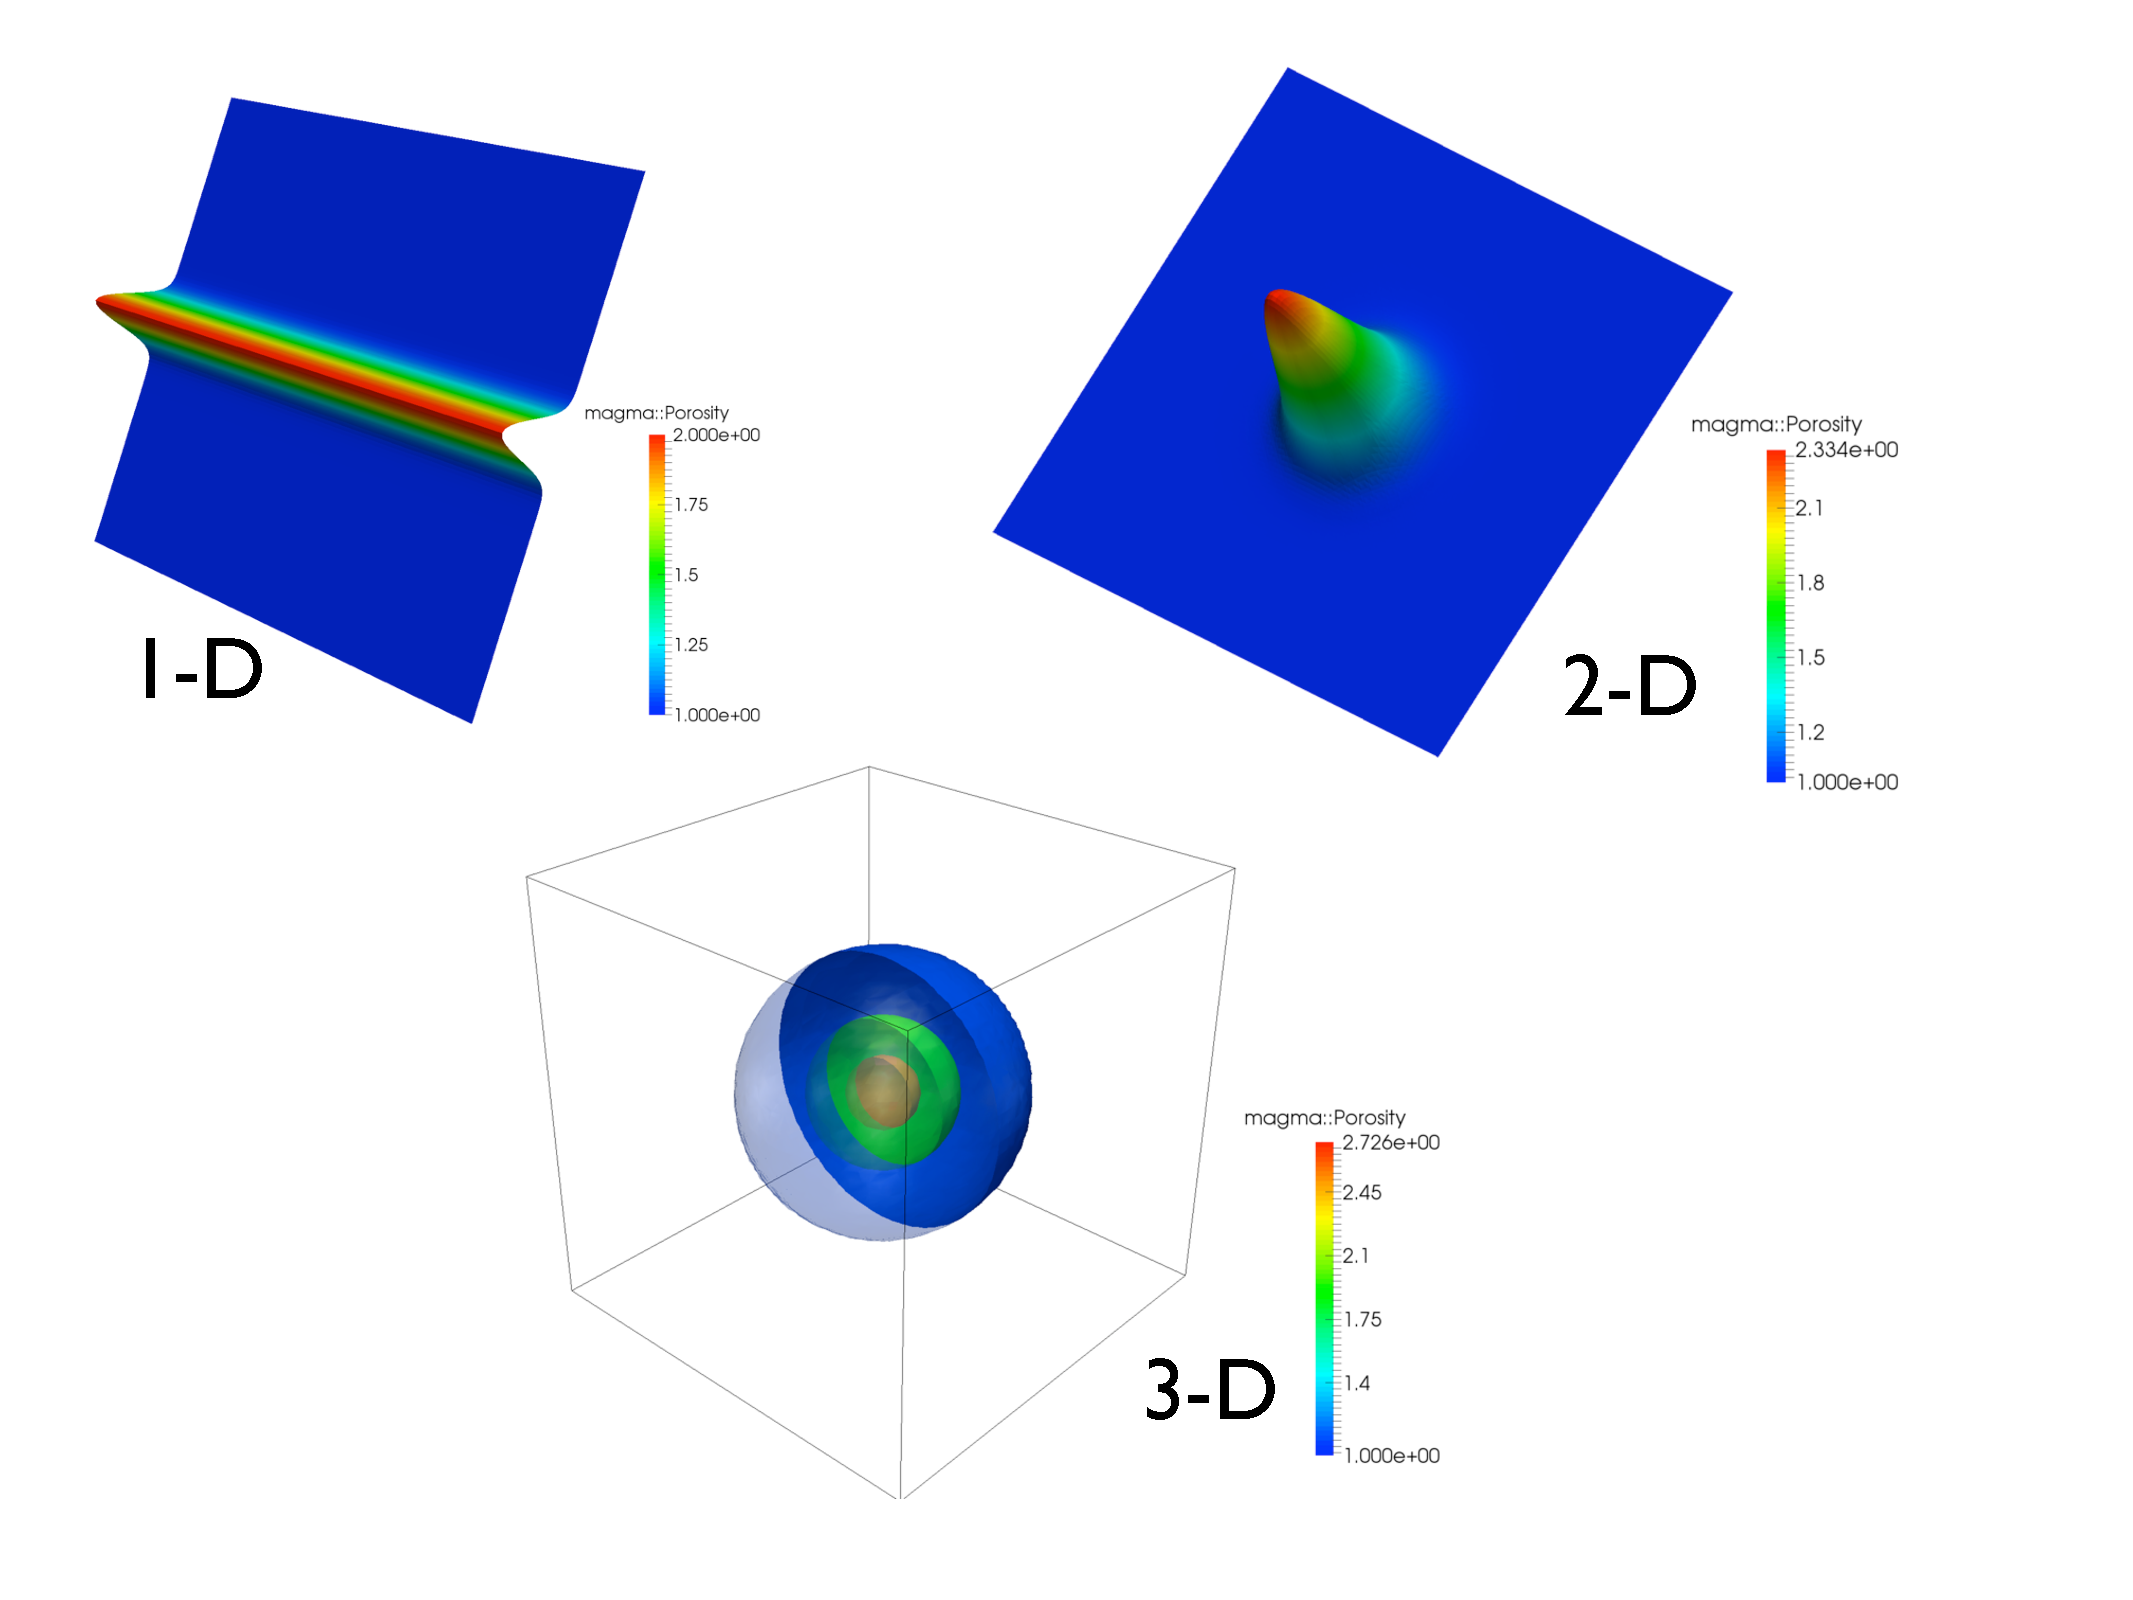
\includegraphics[width=.8\textwidth]{figures/CompositeSolitaryWaves.pdf} 
  \caption{example 1,2 and 3-D magmatic solitary waves that all move
    at speed $c=5$ times the background porosity.}
  \label{fig:SolitaryWavesAllD}
\end{figure}

In the limit of small porosity, the dimensionless governing equations for evolution
of porosity $\phi$ and ``compaction pressure'' $\pcmp$ in a frame
moving at a constant velocity $\Vs$ can be written
\begin{gather}
  \ppt{\phi} + \Vs\cdot\grad\phi = 
  \left(
    \frac{h}{\delta}
  \right)^{2}\frac{\pcmp}{\zeta}  \label{eq:5.1}\\
-\div K \grad\pcmp + \left(
    \frac{h}{\delta}
  \right)^{2}\frac{\pcmp}{\zeta} = \div K \ghat    \label{eq:5.2}
\end{gather}
where $K=\phi^{n}$ is the permeability, $\zeta = 1/\phi^{m}$ is the
bulk viscosity, $\ghat$ is the unit vector in the direction of
gravity.  These equations are scaled by an arbitrary lengthscale $h$
(usually the system height), in which case  $(h/\delta)$ is  the
system height  in compaction lengths
\begin{gather}
  \delta = \sqrt{\frac{K_{0}\zeta_0}{\mu}}
\end{gather}
The compaction length is the intrinsic length scale over which
pressure variations due to obstructions in melt flux propagate as
viscous stresses in the matrix. (See
\cite{spiegelman_flow_1993,spiegelman_flow_1993-1} for more details).

Equations (\ref{eq:5.1})--(\ref{eq:5.2}) for a coupled
hyperbolic/elliptic set of equations for the evolution of porosity and
pressure.  For an arbitrary initial condition, these equations will
break up into a series of localized solitary waves that propagate at a
constant speed that depends on amplitude and maintain constant shape
in the absence of collisions.  Remarkably, however,  we can seek
solitary wave solutions in all dimensions $d$  of the form
\begin{equation}
  \label{eq:5.4}
  \phi(\vec{x},t) = f(r) = f
  \left(
    \sqrt{\sum_{j}^{d-1} x_{j}^{2} + (x_{d} -ct)^{2}}
  \right)
\end{equation}
where $r$ is the radial distance from the peak of the wave.
Substituting $f(r)$ into Equations (\ref{eq:5.1})--(\ref{eq:5.2})
transforms them into a 3rd order, non-linear ODE in $r$.  Except for
some special cases,  these ODE's do not have analytic closed form
solutions, however,  Simpson and Spiegelman
\cite{simpson_solitary_2011}, provides an elegant spectrally accurate
method for numerically calculating solitary wave profiles for all
values of $c,n,m,d$ using the ``sinc collocation method''.  Moreover,
Gideon simpson has encoded this method in a set of python routines
\texttt{magmasinc} which have been included in this tutorial along
with a set of classes for managing and evaluating the solitary wave
profiles.  For example, the script
\texttt{??/??/scripts/see\_solitarywaves.py} initializes 3 different
solitary waves for $c=5$, $n=3$, $m=1$ and $d=[1,2,3]$, using 150
collocation points.  Figure (\ref{fig:SolitaryWaveProfiles}) shows radial profiles $f(r)$ for these
3 waves.  

\begin{figure}[htbp!]
  \centering
  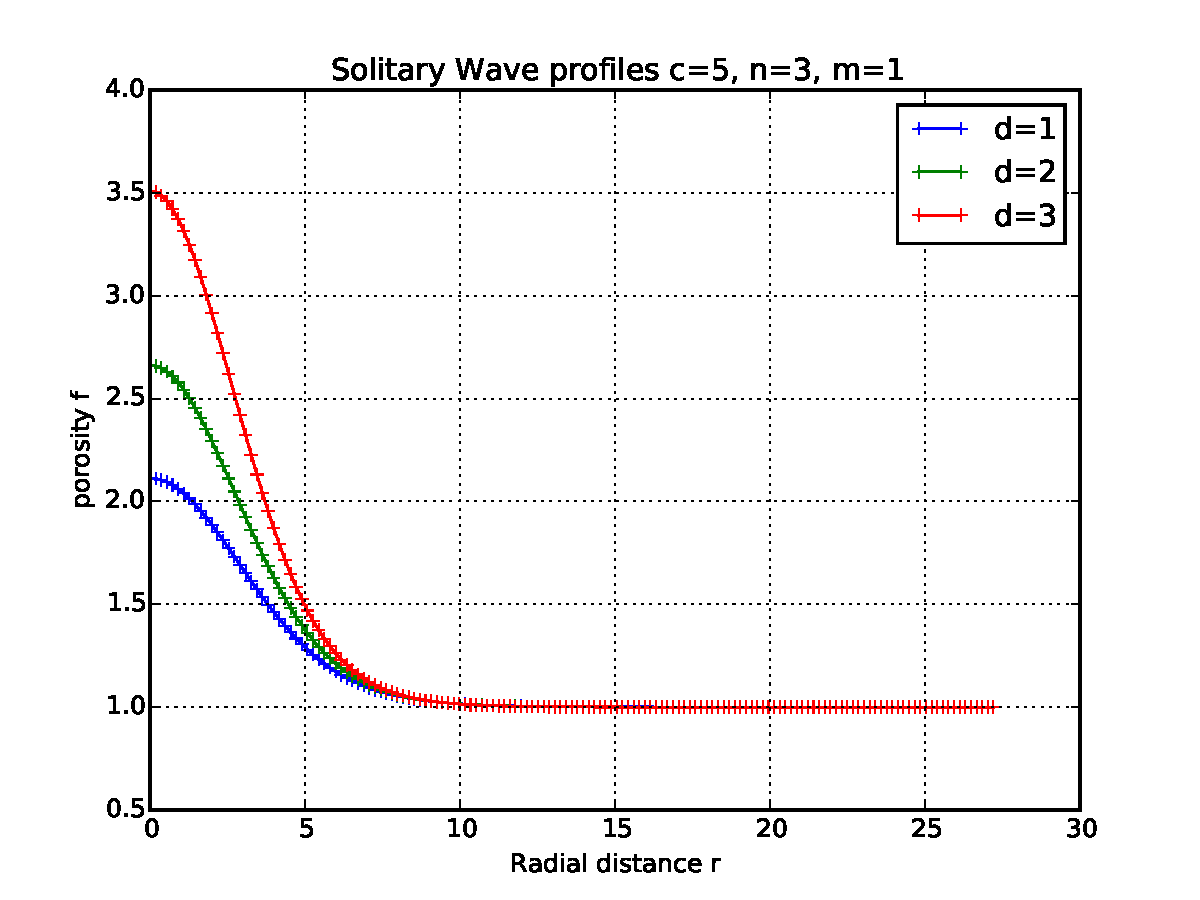
\includegraphics[width=.75\textwidth]{SolitaryWavesProfiles.pdf}
  \caption{Solitary wave profiles $f(r)$ for 1,2 and 3-D waves
    calculated using the pysolwave python package that installs with
    \TF.  All wave travel at speed $c=5$ and have permeability
    exponent $n=3$ and bulk viscosity exponent $m=1$.  Crosses on the
    profiles show the collocation points.}
\label{fig:SolitaryWaveProfiles}
 \end{figure}

\subsection{Benchmark problem}
\label{sec:benchmark-problem}

These solitary waves provide an excellent benchmark problem for
testing any model of multi-phase flow.  If chosen as an initial
condition in a frame moving at speed $\Vs = c\ghat$ they should
simply stay put and not change shape.  Any error in position or shape
is strictly due to numerical errors.  As a first problem we will
explore the solitary wave benchmarks as laid out in Simpson and
Spiegelman, 2011 \cite{simpson_solitary_2011} which have the initial
condition of  a single 2-D
or 3-D wave with its peak at the center of a unit square or cube.
$\Vs$ is set to exactly counter the wave propagation.  Boundary
conditions on porosity and pressure are shown in Figure (\ref{fig:solitarywavebcs}). 

\begin{figure}[htbp!]
  \centering
  \def\svgwidth{.8\textwidth}
  \input{solitaryWaveBCs.pdf_tex}
  \caption{Boundary and initial conditions for the solitary wave
    benchmark problem (Simpson and Spiegelman,\cite{simpson_solitary_2011}}
  \label{fig:solitarywavebcs}
\end{figure}


\subsection{Variational forms and Discontinuous Galerkin Porosity}
\label{sec:variational-forms}

To write out weak forms for Equations (\ref{eq:5.1}) and
(\ref{eq:5.2}) require choosing stable element pairs for porosity and
compaction pressure.  As Eq.\ (\ref{eq:5.2}) is an elliptic equation
in compaction pressure, standard continuous galerkin elements (e.g. \Pone
or \Ptwo) have been shown to be adequate for pressure.  Moreover, In the
absence of the $\Vs\cdot\grad\phi$ term, Eq.\ (\ref{eq:5.1}) is
actually an ODE for porosity and continuous elements are also valid.
However, when the $\Vs\cdot\grad\phi$ is included, Eq.\ (\ref{eq:5.1})
becomes a hyperbolic equation for the evolution of porosity in a frame
moving with the solid which can present significant challenges for
accurate solution using galerkin finite elements.  This term, which
represents advection of porosity by the solid phase is actually
expected for most magma dynamics problems where there is a non-trivial
background flow of solid, such as at a mid-ocean ridge or subduction
zones, and we use it here in the benchmark problem to ``freeze'' the
solitary wave in the box by having the background flow exactly balance
the wave speed $c$.  After some trial and error, we found that using
discontinuous Galerkin elements for Porosity, worked fine.  Here we
will use the mixed discrete function space $\fspace=(\Ptwo,\Ptwodg)$
where $\vec{u}\in\fspace=(p,f)$ (where $p$ will be our  \texttt{ufl}
symbol for pressure and $f$ for porosity $\phi$).

As with the energy equation in thermal convection, we will first
discretize the time derivative in the porosity equation using finite
differences and integrate using a $\theta$ scheme.  
Multiplying by appropriate test functions and integrating by parts, the
variational form of the non-linear problem can be written
\begin{quote}
  \fbox{\parbox{.9\textwidth}{Find $\vec{u}\in \fspace$ such that
      \begin{equation}
         F(\vec{u};\vec{u}_{t}) =0 
      \end{equation}
  for all test functions $\vec{u}_{t}=(p_{t},f_{t}) \in\fspace$.}}
\end{quote}
 where $F(\vec{u};\vec{u}_{t}) = F_{p} + F_{f}$ with
\begin{align}
         F_{p} =  & \int_\Omega \left[\dot{\epsilon}(\vec{v}_{t}):
             2\eta \dot{\epsilon}(\vec{v}_{i}) -
             p_{i}\div\vec{v}_t  - T_{i}\vec{v}_{t} \cdot\vec{k} \right]d\vec{x}  \\
 F_{f} =& -\int_\Omega p_t\div\vec{v}_{i} d\vec{x}\\
\label{eq:5.5}\\
\nonumber \\
  F = & F_{p} + F_{f} \label{eq:5.systemresidual}
\end{align}
where 
\begin{align*}
  f_{\theta} = & (1-\theta)f_{n} + \theta f_{i}\\
  \Vs_{\theta} = & (1-\theta)\Vs_{n} + \theta \Vs_{i}
\end{align*}
are $\theta$ weighted variables.  As before here we use $\theta=1/2$.

\section{Solution using \TF}
\label{sec:solution-using-tf}



%\pagebreak{}
\section{Themes and Variations}
\label{sec:themes-variations}


\subsection{Variable Viscosity}
\label{sec:variable-viscosity}


%%% Local Variables: 
%%% mode: latex
%%% TeX-master: "tftutorials"
%%% End: 
